\section{Where the uniform step could come from}\label{cp:sec:uniform}

Section~\ref{sec:ch25:open} names three mechanisms that could supply the missing uniform step: a positive approximating family whose positivity is proved independently, a Hilbert P\'olya operator, or a direct Weil inequality.

\subsection{The Weil Gram matrix on compactly supported test functions}\label{cp:sec:weil}

For $h$ smooth enough, even or not (each term depends on $h$ only through its even part $h_e$, defined below), with $\hat h(r)=\int h(x)e^{irx}\,dx$, the explicit formula reads
\[\begin{aligned}
\sum_\rho\hat h(\gamma_\rho)&=\hat h(\tfrac i2)+\hat h(-\tfrac i2)-\sum_{n\ge2}\frac{\Lambda(n)}{\sqrt n}\big(h(\log n)+h(-\log n)\big)\\&\qquad+\frac1{2\pi}\int_\R\hat h(r)\,\re\psi\big(\tfrac14+\tfrac{ir}2\big)\,dr-h(0)\log\pi,
\end{aligned}\]
with $\rho=\frac12+i\gamma_\rho$ and $\psi=\Gamma'/\Gamma$. For $h=g*\tilde g$ with $\tilde g(x)=\overline{g(-x)}$ and $g$ supported in $[-L/2,L/2]$, the left side is $\sum_\rho|\hat g(\gamma_\rho)|^2\ge0$ under RH, which is Weil's criterion \cite{Weil52}, $h$ is supported in $[-L,L]$, and the prime sum runs over prime powers $n\le e^L$. The archimedean term was evaluated in $x$ space,
\[\begin{gathered}
\frac1{2\pi}\int\hat h(r)\,\re\psi\big(\tfrac14+\tfrac{ir}2\big)\,dr=\int_0^\infty\Big[\frac{h(0)e^{-2x}}x-\frac{2h_e(x)e^{-x/2}}{1-e^{-2x}}\Big]dx,\\ h_e(x)=\tfrac12\big(h(x)+h(-x)\big),
\end{gathered}\]
which is far better conditioned than the $r$ integral for compactly supported $h$: truncated at $r=400$, the $r$ integral carries an error of $6\times10^{-6}$ in the archimedean term of the diagonal entry at $w=0.1$, more than two thousand times the smallest eigenvalue $2.5\times10^{-9}$ of Table~\ref{cp:tab:weil}. With hat functions $g_j(x)=\max(0,1-|x-c_j|/w)$ at nodes spaced $w$ apart inside $[-L/2,L/2]$, $N=L/w-1$ functions in all, $h_{jk}=g_j*\tilde g_k$ is an explicit piecewise cubic, and the Gram matrix $G_{jk}=W(h_{jk})$ is Hermitian, with $W(g*\tilde g)\ge0$ on the span exactly when $G$ is positive semidefinite.

\begin{table}[ht]
\centering\small
\begin{tabular}{@{}rrrrrl@{}}
\toprule
$w$ & $L$ & $N$ & $\lambda_{\min}$ & $\lambda_{\max}$ & pole, $-$prime, archimedean\\
\midrule
$0.25$ & $1$ & $3$ & $4.22\times10^{-4}$ & $0.034$ & $0.3468,\ -0.0141,\ -0.3322$\\
$0.25$ & $2$ & $7$ & $2.22\times10^{-5}$ & $0.050$ & $0.8410,\ -0.2472,\ -0.5938$\\
$0.25$ & $4$ & $15$ & $4.70\times10^{-7}$ & $0.096$ & $1.6494,\ -0.8550,\ -0.7944$\\
$0.25$ & $6$ & $23$ & $3.56\times10^{-8}$ & $0.144$ & $2.7255,\ -1.8067,\ -0.9187$\\
$0.1$ & $1$ & $9$ & $1.84\times10^{-5}$ & $0.083$ & $0.1287,\ -0.0019,\ -0.1268$\\
$0.1$ & $2$ & $19$ & $1.27\times10^{-6}$ & $0.149$ & $0.2900,\ -0.0676,\ -0.2224$\\
$0.1$ & $4$ & $39$ & $5.70\times10^{-8}$ & $0.290$ & $0.7281,\ -0.3981,\ -0.3300$\\
$0.1$ & $6$ & $59$ & $2.48\times10^{-9}$ & $0.431$ & $1.1050,\ -0.7353,\ -0.3697$\\
\bottomrule
\end{tabular}
\caption{The Weil Gram matrix on hat functions. The last column splits $\lambda_{\min}=v^*Gv$ for the minimising unit vector into the pole, prime (with its sign) and archimedean pieces. Script \texttt{phase\_weil.py}, output \texttt{phase\_weil.json}.}
\label{cp:tab:weil}
\end{table}

\begin{table}[ht]
\centering\small
\begin{tabular}{@{}rrrrl@{}}
\toprule
$w$ & $L$ & $\lambda_{\min}$ (arithmetic) & $\sum_\rho|\hat g(\gamma_\rho)|^2$ (zeros) & zeros carrying most of the sum\\
\midrule
$0.25$ & $1$ & $4.2184\times10^{-4}$ & $4.2184\times10^{-4}$ & \#2 ($56\%$), \#4 ($20\%$), \#5 ($11\%$)\\
$0.25$ & $3$ & $1.8238\times10^{-6}$ & $1.8237\times10^{-6}$ & \#9 ($44\%$), \#11 ($24\%$), \#20 ($5\%$)\\
$0.25$ & $6$ & $3.5562\times10^{-8}$ & $3.5560\times10^{-8}$ & \#10 ($40\%$), \#20 ($13\%$), \#30 ($9\%$)\\
$0.1$ & $2$ & $1.2691\times10^{-6}$ & $1.2691\times10^{-6}$ & \#13 ($37\%$), \#15 ($15\%$), \#16 ($15\%$)\\
$0.1$ & $4$ & $5.7008\times10^{-8}$ & $5.7004\times10^{-8}$ & \#14 ($36\%$), \#13 ($23\%$), \#16 ($7\%$)\\
$0.1$ & $6$ & $2.4846\times10^{-9}$ & $2.4841\times10^{-9}$ & \#41 ($32\%$), \#15 ($17\%$), \#14 ($8\%$)\\
\bottomrule
\end{tabular}
\caption{The smallest eigenvalue from the arithmetic side against the sum of squares of $\hat g_{\min}$ over the first $1500$ zeros, with the zeros (by index) that carry the largest shares. Script \texttt{phase\_weil.py}, output \texttt{phase\_weil.json}.}
\label{cp:tab:weilcheck}
\end{table}

\begin{figure}[ht]
\centering
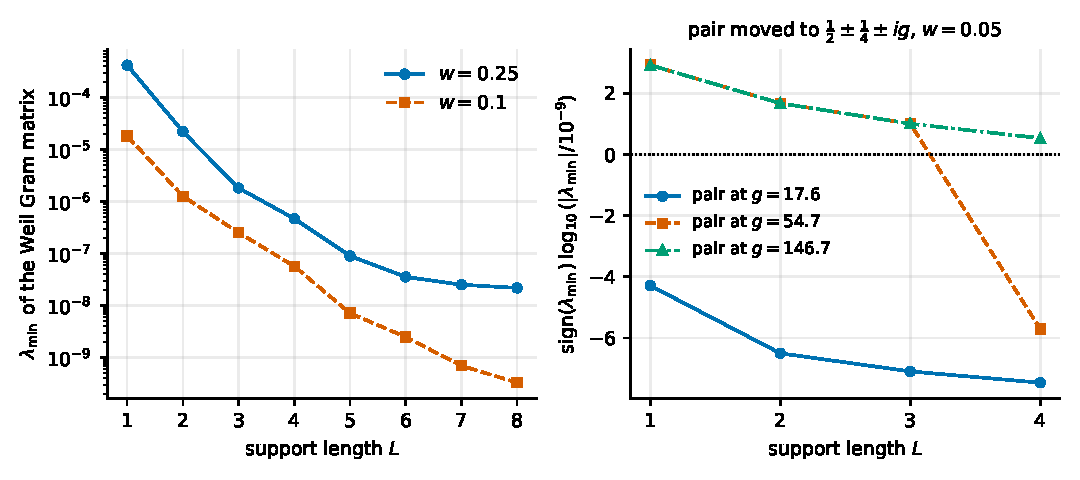
\includegraphics[width=\textwidth]{fig/cp_weil.pdf}
\caption{Left: $\lambda_{\min}$ of the Weil Gram matrix against the support length $L$ for two resolutions. Right: a pair of zeros at height $g$ moved to the quadruple $\frac12\pm\frac14\pm ig$, signed logarithm of $\lambda_{\min}$ for $w=0.05$. The pair at $g\approx17.6$ is detected at every $L$, the pair at $g\approx54.7$ only at $L=4$, and the pair at $g\approx146.7$ not at all within $L\le4$. Script \texttt{phase\_weil.py}, output \texttt{phase\_weil.json}.}
\label{cp:fig:weil}
\end{figure}

The experiment says three things (Tables~\ref{cp:tab:weil} and~\ref{cp:tab:weilcheck}, Figure~\ref{cp:fig:weil}). First, $\lambda_{\min}>0$ throughout and it falls roughly geometrically in $L$, by a factor between about $2.5$ and $20$ per unit of $L$ up to $L=6$, as it must, since the nodes are nested (for the values of $L$ used), so that the matrix for a shorter support is a principal submatrix of the matrix for a longer one, and the smallest eigenvalue of the Weil form on $[-L/2,L/2]$ tends to zero as $L$ grows: a long enough support can make $\hat g$ small at every low ordinate. Second, the two sides of Weil's identity agree to a relative $2\times10^{-4}$ at every $(w,L)$, down to $\lambda_{\min}=2.5\times10^{-9}$; and the margin is carried by a handful of zeros, zero $41$ at height $124.3$ carrying $32\%$ at $w=0.1$, $L=6$. Third, at $w=0.05$ a pair displaced at height $g\approx17.6$ makes $\lambda_{\min}$ negative at every $L\le4$, one at $g\approx54.7$ only at $L=4$ and one at $g\approx146.7$ at no $L\le4$, an instance of the finite information principle of Section~\ref{cp:sec:finiteinfo}. How fine $w$ must be to see a pair at height $g$ is not fixed by one resolution: at $w=0.2$ the pair at $g\approx17.6$ is already seen at $L=2$, with $wg\approx3.5$.

The sign structure is the reverse of the L\'evy picture of Section~\ref{ch:basepoint}, where the pole of $\zeta$ is a negative input to $\log\xi$; in the Weil form the pole, on the minimising vectors of Table~\ref{cp:tab:weil}, contributes positively. A certificate for the Weil form would therefore have to show, for every $L$, that the three terms together are nonnegative on the whole span, although the pole term alone is not (for real odd $g$ it is $-2G(\frac12)^2$, with $G(a)=\int g(x)e^{ax}\,dx$), and on the minimising vectors the pole term outweighs the prime and archimedean terms only by a margin that tends to zero. No uniformly positive quadratic form can do that. What could is a factorisation $W(g*\tilde g)=\|Ag\|^2$ with $A$ built from the arithmetic and exact positivity, the shape of the Hilbert P\'olya mechanism, and Problem~\ref{cp:prob:chol} asks for the first experiment in that direction.

\subsection{The zero gas along the flow}\label{cp:sec:gas}

In the variable $z=2\gamma$ the zeros of $H_t$ move, while simple, by $dz_k/dt=2\sum_{j\ne k}(z_k-z_j)^{-1}$ (Section~\ref{sec:ch21:flow}, with five of the zeros at four times in Table~\ref{tab:ch21:flowzeros}). We integrated this system for the first $600$ zeros, heights up to $939.02$, with a frozen tail for the omitted zeros (the zeros $601$ to $1700$ held at their positions at $t=0$ and a continuum of density $\frac1{4\pi}\log(z/4\pi)$ beyond them, whose drift on $z_k$ is $-4z_k\sum_{j>600}z_j^{-2}$ to leading order), backward from $t=0$ until the first gap fell below $0.02$ and forward to $t=0.3$. Along the trajectory we recorded the minimum normalised gap $s_{\min}(t)=\min_k(z_{k+1}-z_k)\frac1{4\pi}\log(z_{k+1}/4\pi)$ and the Csordas, Smith and Varga quantity $\min_k\Delta_k^2g_k$ over the first $400$ pairs, with $\Delta_k=z_{k+1}-z_k$ and $g_k=\sum_{j\ne k,k+1}[(z_k-z_j)^{-2}+(z_{k+1}-z_j)^{-2}]$, where $j$ runs over all the other zeros $\pm z_j$ of the model, the frozen tail and the continuum included; a pair with $\Delta_k^2g_k<\frac45$ is a Lehmer pair in the sense of \cite{CSV94} and Section~\ref{sec:ch21:bounds}.

\begin{figure}[ht]
\centering
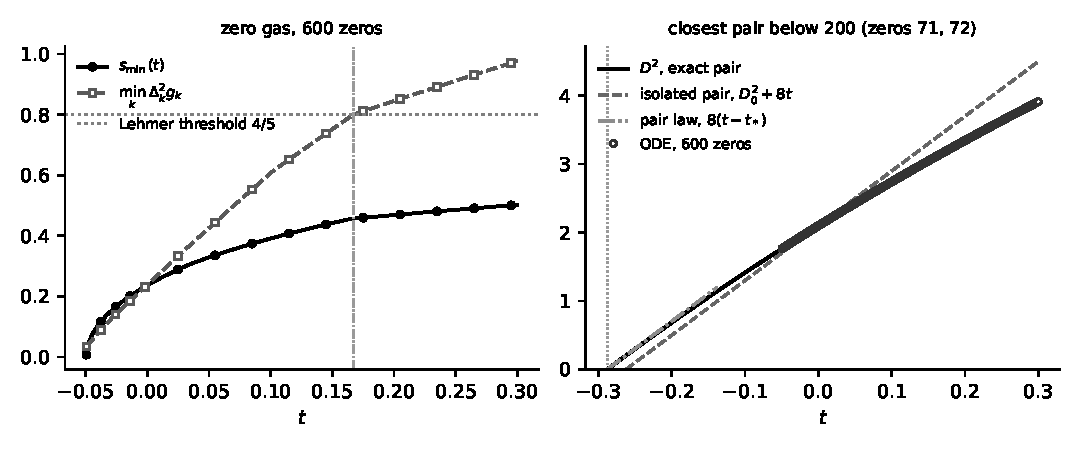
\includegraphics[width=\textwidth]{fig/cp_flow.pdf}
\caption{Left: the minimum normalised gap and $\min_k\Delta_k^2g_k$ along the flow, both monotone on the computed range; the second crosses the Lehmer threshold $\frac45$ near $t=0.17$. Right: $D^2$ for the closest pair below height $200$, at ordinates $184.87$ and $185.60$, against the isolated pair law $D_0^2+8t$.}
\label{cp:fig:flow}
\end{figure}

\begin{proposition}[Computed; the upper end of (iii) certified]\label{cp:prop:gas}
(i) The backward integration stops at $t=-0.0493$, when the pair at ordinates $750.656$ and $750.966$, the $453$rd and $454$th zeros, collides; the isolated pair estimate is $-D_0^2/8=-0.048$. (ii) At the $171$ times sampled in $[-0.049,0.30]$ both $s_{\min}(t)$ and $\min_k\Delta_k^2g_k$ are strictly increasing, from $0.0076$ to $0.502$ and from $0.035$ to $0.977$; at $t=0$ the minimiser of $\Delta_k^2g_k$ is the pair at $564.16$ and $564.51$, with value $0.238$. (iii) For the pair near $185$, the pair $(\gamma_{71},\gamma_{72})$ of Section~\ref{sec:ch21:collisions}, certified signs of $\xi_t(\frac12+i\theta)$ in Arb at $640$ bits (the trapezoid sum of Section~\ref{sec:ch4:trapezoid} with an enclosure of its discretisation error) at $131$ points of $[184.6,185.9]$, with bisection in $t$ on the number of sign changes, show that the pair is still real at $t=-0.287979$, and with the pair law below place the collision in $[-0.28803,-0.287979]$, in agreement with the value $-0.2880$ of Section~\ref{ch:dbn} and inside the bracket of Section~\ref{sec:wigbiane:brackets}. Newton's method on the same sum puts the double zero at $z_*=370.78087$, $t_*=-0.287979837009$; a Krawczyk test certifies a real double zero of the trapezoid sum itself in a box of half width $2^{-400}$ about this point (a statement about the sum, not about $H_t$), and at $t=t_*+1.2\times10^{-12}$ the signs $+,-,+$ of $H_t$ at $z_*-4\times10^{-6}$, $z_*$ and $z_*+4\times10^{-6}$ show that the pair is still real, which certifies that the collision lies below $-0.287979837008$: the upper end of the bracket is certified and the lower end is not. The extrapolation of the integrated $D^2$ was $7\%$ early and the isolated pair estimate $-0.262$ was $9\%$ late. Script \texttt{phase\_gas.py} for (i) and (ii), output \texttt{phase\_gas.json}; script \texttt{phase\_collide.py} for (iii), output \texttt{phase\_collide.json}.
\end{proposition}

The bracket in (iii) uses that a pair at distance $D$ in $z$ obeys $D^2\approx8(t-t_*)$ near the collision (Section~\ref{sec:ch21:collisions}), so sign changes on a grid of step $0.01$ in $\theta$ vanish at most $0.01^2/2=5\times10^{-5}$ above $t_*$. At $t=-0.287981$ the grid finds none, which does not exclude two real zeros less than $0.01$ apart, and the lower end rests on the pair law, an asymptotic statement and not an enclosure.

The question is whether a gap functional, monotone as in (ii), can carry a positive lower bound from $t>0$ down to $t=0$ uniformly in the height, and the data suggest that gap functionals cannot. Both are minimised at Lehmer pairs, whose normalised gaps are expected, on the GUE conjecture, to be arbitrarily small at large height, so their infimum over all heights would be zero at $t=0$. A Lyapunov functional for RH must be global, insensitive to individual close pairs, in the manner of the pair correlation that Rodgers and Tao used to prove the reverse inequality \cite{RodgersTao}; we did not find a candidate. Two rigorous companions of the data are in Sections~\ref{nw:sec:shield} and \ref{sec:ft:persist}: an exact formula for the drift of a gap, and a proof that no bound through the absolute value of the integrand gives a step uniform in the height \cite{Newton26}.

\subsection{The cost of the flow route}\label{cp:sec:cost}

The published points of the phase diagram give the cost of descending along it (Table~\ref{tab:ch21:hist} lists the bounds on $\Lambda$). Polymath15 proved $\Lambda\le0.22$ with the barrier $X\approx6\times10^{10}$, and Table~1 of their paper lists, for each bound from $\Lambda\le0.21$ down to $\Lambda\le0.1$, the barrier $X$ that the same method needs, with RH verified to height $X/2$ \cite{Polymath}: $X\approx2\times10^{12}$ for $0.21$, $5\times10^{12}$ for $0.2$, $2\times10^{13}$ for $0.19$, $7\times10^{15}$ for $0.15$ and $9\times10^{21}$ for $0.1$. Platt and Trudgian obtained $\Lambda\le0.2$ from the second row, which by their account needs verification to $2.51\times10^{12}$, and the third row, $0.19$, requires verification slightly above $10^{13}$ \cite{PT21}. The product $\Lambda\log X$ is $5.46$ at $0.22$ and falls along the table from $5.95$ at $0.21$ to $5.06$ at $0.1$.

\begin{proposition}[Computed]\label{cp:prop:cost}
The least squares fit of $\Lambda=c/\log X$ in $1/\log X$ to the bound $\Lambda\le0.22$ and the twelve rows of the table gives $c=5.59$, with residuals below $0.013$ in $\Lambda$, which along the table are errors of up to a factor of about $200$ in $X$; on this law a bound $\Lambda\le\delta$ requires a barrier $X$ of order $e^{c/\delta}$, that is verification to height $X/2$: $X=10^{48.6}$ for $\delta=0.05$ and $10^{242.9}$ for $\delta=0.01$. Since $\Lambda\log X$ falls along the table, the law $\log X=a/\Lambda+b$ fits its twelve rows better, with $a=4.24$, $b=8.28$ and residuals below $0.003$ in $\Lambda$, within a factor $1.6$ in $X$, and gives $X=10^{40.4}$ for $\delta=0.05$ and $10^{187.7}$ for $\delta=0.01$. Script \texttt{phase\_scaling.py}, output \texttt{phase\_scaling.json}.
\end{proposition}

\begin{figure}[ht]
\centering
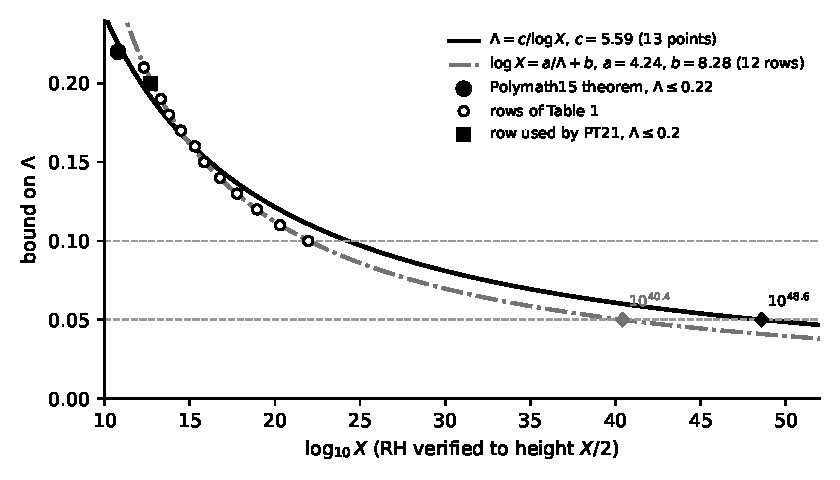
\includegraphics[width=0.78\textwidth]{fig/cp_scaling.pdf}
\caption{The bound $\Lambda\le0.22$ of Polymath15 and the twelve rows of their table of conditional bounds \cite{Polymath} against the barrier $X$ (verification height $X/2$), with the fits $\Lambda=c/\log X$ and $\log X=a/\Lambda+b$. Dashed lines mark $\Lambda=0.1$ and $0.05$.}
\label{cp:fig:scaling}
\end{figure}

Beyond the table the two laws should be read as orders of magnitude. Their form agrees with the heuristic that the flow at time $t$ makes the zeros near height $x$ real once $t\log x$ exceeds a constant, which is how the Riemann Siegel type approximation of $H_t$ enters \cite{Polymath}. Along the table, halving the bound from $0.2$ to $0.1$ raises the required barrier from $5\times10^{12}$ to $9\times10^{21}$, to about its power $1.7$, and the power is $2$ at every bound on the law $c/\log X$ and tends to $2$ as the bound decreases on the law $\log X=a/\Lambda+b$. By the table itself the bound $\Lambda\le0.15$ needs verification to a height of about $3.5\times10^{15}$, some $1200$ times the record $3\times10^{12}$ \cite{PT21}, and $\Lambda\le0.1$ about $4.5\times10^{21}$; no conceivable computation reaches $0.05$. The flow route produces a theorem at every stage, a monotone sequence of upper bounds for $\Lambda$, which is $0$ exactly when RH holds \cite{RodgersTao}, as no other route does, and it cannot reach the corner of the diagram by computation.

\subsection{A programme}\label{cp:sec:programme}

The phase diagram suggests five steps, of which the first three are engineering.
\begin{enumerate}
\item An evaluator: a Riemann Siegel type form of $\xi_t$ and $\xi_t'$, such as the effective approximation of $H_t$ in \cite{Polymath}, in ball arithmetic, at a cost of about $\sqrt{\theta/2\pi}$ terms per point (Table~\ref{tab:compare}), replacing the P\'olya integral, whose required precision grows like $0.341\,\theta$ digits (Section~\ref{sec:ch4:trapezoid}); see Section~\ref{st:sec:wp2} for $t=0$.
\item Certificates in Thorin form: Theorem~\ref{cp:thm:cert} or Proposition~\ref{cp:prop:thorincert} at a target $(t_0,\alpha_0)$ up to the barrier.
\item The tail in the same framework: the barrier and the analytic region beyond it \cite{Polymath}, so that the points of Corollary~\ref{cp:cor:known}(b) and (c) are certified end to end and stated as GGC theorems.
\item A measurement: the optimal $(t_0,\alpha_0)$ on each level set as a function of the verification height, and the constant $c$ of Proposition~\ref{cp:prop:cost} as a function of the height.
\item The structural step: a tail at $t=0$ below the basepoint $\frac78$. Every certified point is a theorem, and by Proposition~\ref{cp:prop:see} no computed window distinguishes the corner from them; the step is the existence of the tail, and it must come from one of the mechanisms of Section~\ref{sec:ch25:open}.
\end{enumerate}

\subsection{Open problems}\label{cp:sec:open}

\begin{problem}\label{cp:prob:high}
Compute $v_t(\alpha,\theta)$ at $t=0$ and $t=0.2$ near the Polymath barrier, heights near $3\times10^{10}$, with a Riemann Siegel type evaluator of $H_{0.2}$ such as the effective approximation of \cite{Polymath} (Section~\ref{ch:classical} gives the one for $\zeta$), and measure how the difference between the functions $v_{0.2}/\pi$ and $v_0/\pi$ grows with the height. Proposition~\ref{cp:prop:see}(iii) measures it below $100$. For $t=0$ see work package~2 of Section~\ref{st:sec:wp2} and Section~\ref{sec:ch25:contrib}.
\end{problem}

\begin{problem}\label{cp:prob:boundary}
Describe the boundary $\alpha^*(t)$ of $\mathcal G$ for $0\le t\le0.2$ as far as computation and the known zero free regions allow. Is $\alpha^*$ continuous, and is $(\alpha^*(t)-\frac12)^2+\frac t2$ strictly decreasing in $t$ where $\alpha^*(t)>\frac12$? Theorem~\ref{cp:thm:phase}(i) shows that it is nonincreasing there. Problem~\ref{mw:prob:flow} asks the neighbouring question for the flow clock $T_t$, $0<t<0.2$.
\end{problem}

\begin{problem}\label{cp:prob:trunc}
Give the symmetrised truncations of Section~\ref{ch:rz4} a coordinate on the phase diagram: for some $(t,\alpha)$ outside the region of Corollary~\ref{cp:cor:known}, is there a family of explicit truncations of $\xi_t$, built from finitely many terms of the P\'olya integral or of a Dirichlet series and making no use of the zeros, as the symmetrised lattice truncations $K_n$ of Subsection~\ref{rz:sec:finite} are, that converges to $\xi_t$ on compact sets, together with heights $h_n\to\infty$ such that for infinitely many $n$ the truncation has no zero with $\re s>\alpha$ and $|\im s|<h_n$? Hurwitz's theorem then makes $(t,\alpha)$ a new point of $\mathcal G$, as in Corollary~\ref{mw:cor:hurwitz}(c); at $t=0$ and $\alpha=\frac12$ the question for the $K_n$ is Conjecture~S (Theorem~\ref{rz:thm:symhurwitz}), and for the stages of Chapter~\ref{chap:maxwald} it is Problem~\ref{mw:prob:hurwitz}.
\end{problem}

\begin{problem}\label{cp:prob:chol}
Compute the Cholesky factor of the Weil Gram matrix of Section~\ref{cp:sec:weil} for decreasing $w$ and increasing $L$, and decide whether its entries converge to an object built from the arithmetic, the first test of a factorisation $W(g*\tilde g)=\|Ag\|^2$.
\end{problem}

\begin{problem}\label{cp:prob:gas}
Find a global functional of the zeros of $H_t$, insensitive to individual close pairs, that is monotone along the flow and whose positivity at $t=0$ excludes collisions at positive time. Biane's gap functional of Section~\ref{sec:wigbiane:biane} is local, the minimum over one gap of Laguerre's quantity, and Problems~\ref{prob:wigbiane:control} and~\ref{prob:wigfree:collide} ask for the control of the nonreal zeros that would make its brackets unconditional; the functional asked for here should instead be one quantity for all the zeros.
\end{problem}

\subsection*{Notes}

The phase diagram theorem is de Bruijn's strip theorem \cite[Theorem 13]{deBruijn} read through Theorem~\ref{cp:thm:transfer}; its case $t=0$ is in Section~\ref{ch:dbn}. Theorem~\ref{cp:thm:transfer}, the certificate of Section~\ref{cp:sec:cert} with Theorem~\ref{cp:thm:rig}, and the experiments of Sections~\ref{cp:sec:weil} and~\ref{cp:sec:gas} are from the authors' working report \cite{FA26}. The bounds on $\Lambda$ are those of de Bruijn \cite{deBruijn}, Ki, Kim and Lee \cite{KKL09}, Polymath15 \cite{Polymath} and Platt and Trudgian \cite{PT21}, and the lower bound is Rodgers and Tao \cite{RodgersTao}. The half plane $\re s>\frac78$ is the announcement \cite{OAI26a}, discussed in Section~\ref{sec:ch25:open}. The description of the Thorin measure as one object with a prime face and a zero face, joined by the sine squared lemma, is developed for automorphic $L$ functions in \cite{LG26}.
